Using data from \gls{cordis}, the structures of five European research projects that are part of the \gls{h2020} programme were analysed.
The selected projects are:
\begin{enumerate}
    \item ``BIM-based holistic tools for Energy-driven Renovation of existing Residences''\label{project1}
    \item ``Integrated and Replicable Solutions for Co-Creation in Sustainable Cities''
    \item ``New integrated methodology and Tools for Retrofit design towards a next generation of ENergy efficient and sustainable buildings and Districts''
    \item ``Proactive synergy of inteGrated Efficient Technologies on buildings' Envelopes''
    \item ``Adaptive Multimodal Interfaces to Assist Disabled People in Daily Activities'' 
\end{enumerate}

All five projects analyzed follow the same structural format, including their data organization, key components, and reporting style.
Due to this uniformity, providing a detailed analysis for each project would be redundant.
Therefore, to avoid repetition and ensure clarity, only the analysis of Project \ref{project1} is presented below as a representative example.

\subsubsection*{BIM-based holistic tools for Energy-driven Renovation of existing Residences}

The BIMERR project, funded under the Horizon 2020 program, aims to develop BIM-based holistic tools for energy-driven renovation of existing residential buildings.
This research initiative focuses on digital transformation in the construction sector, particularly in building renovation, by enhancing \gls{bim} interoperability and streamlining the renovation workflow.
The project is structured around three main pages: Fact Sheet, Reporting, and Results, each of which has a distinct purpose in presenting project details, progress, and outcomes.

\paragraph*{Fact Sheet.}
It provides an overview of the BIMERR project, including its duration, objectives, keywords, programmes, topics, call for proposal, sub call, funding schemes, and consortium partners.
The project, officially titled ``BIM-based holistic tools for Energy-driven Renovation of existing Residences'', as shown in Fig.~\ref{fig:bimerr-fact-sheet}, was coordinated by Fraunhofer Gesellschaft zur F\"orderung der Angewandten Forschung EV in Germany.

\begin{figure}[htbp]
    \centering
 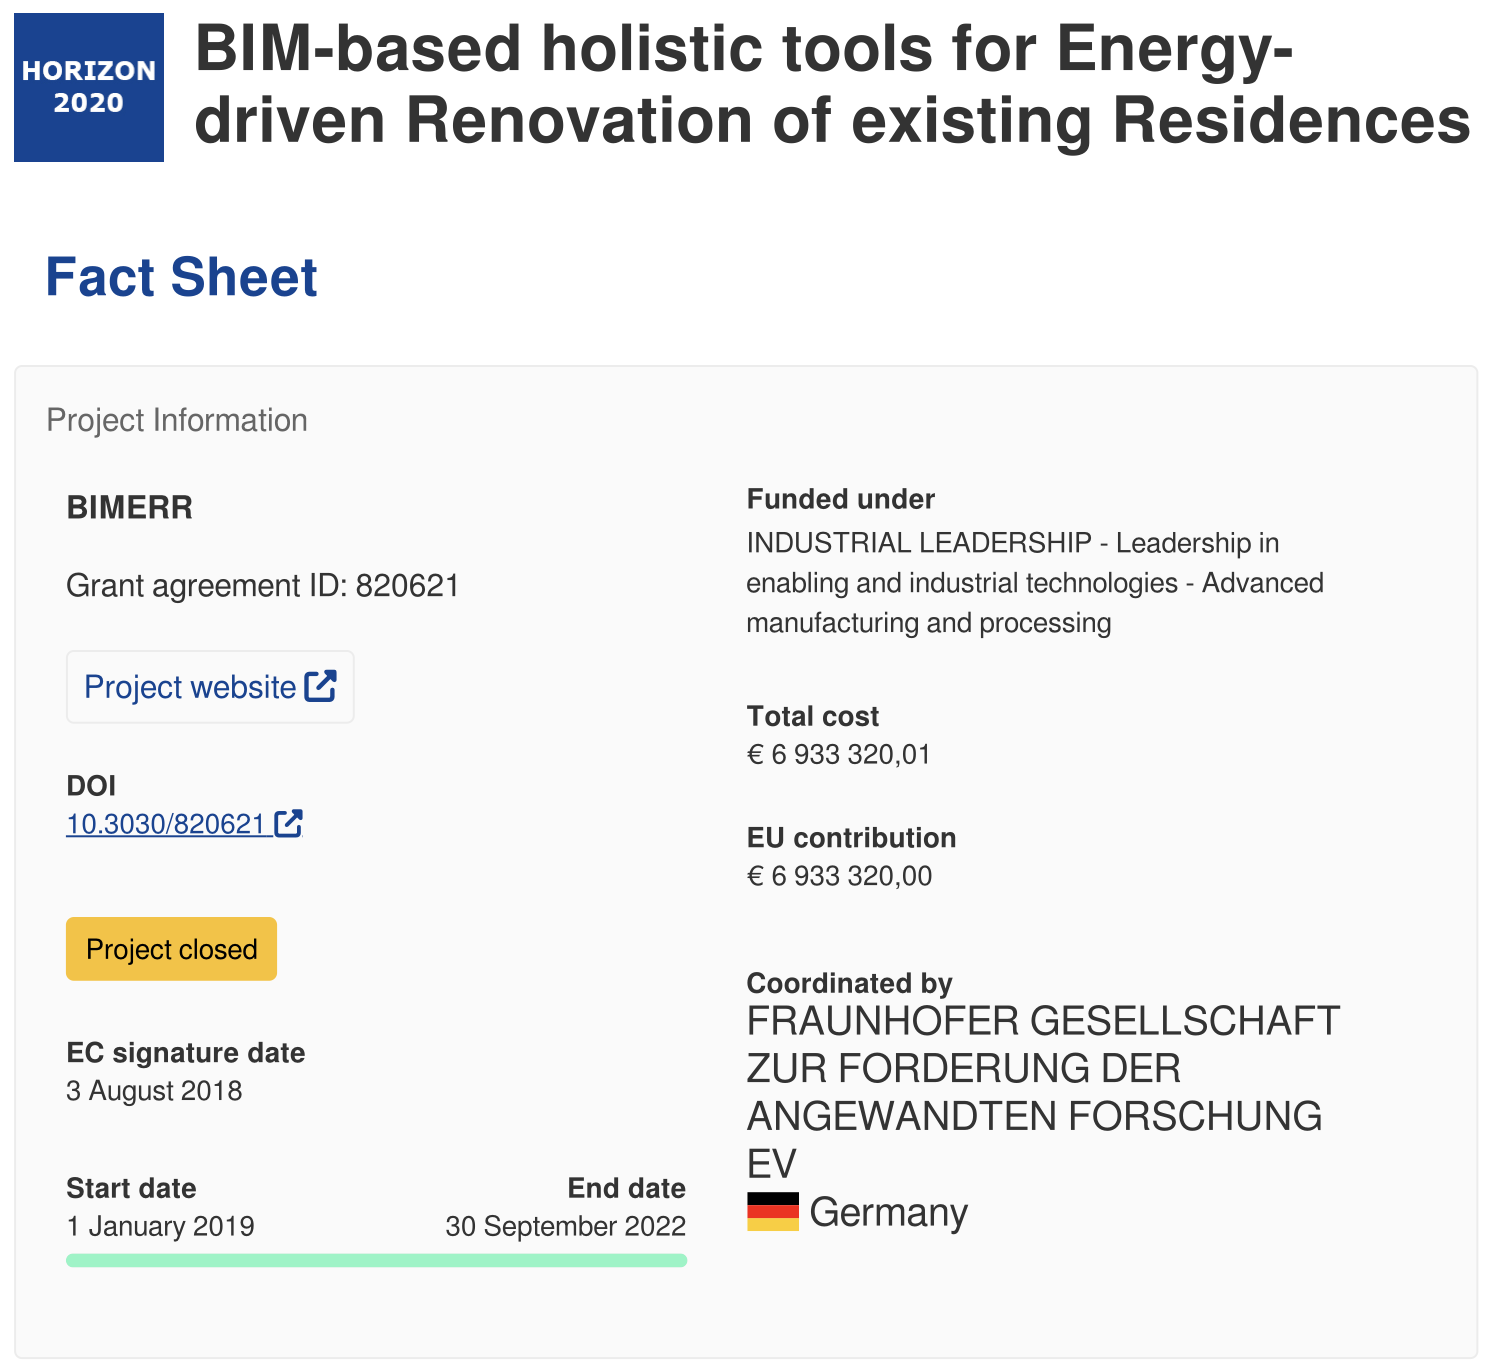
\includegraphics[width=.9\textwidth]{figures/scenario-analysis/bimerr-fact-sheet.png}
     \rule{35em}{0.5pt}
    \caption{BIMERR Project Fact Sheet}
 \label{fig:bimerr-fact-sheet}
\end{figure}

The project ran from January 1, 2019, to September 30, 2022, with a total cost of \euro 6,933,320.01, fully funded by the EU.
The Fact Sheet highlights BIMERR's key mission: developing an ICT-enabled Renovation 4.0 framework, which includes enhanced digital models of existing buildings that integrate geometrical, material, and operational data.
These models support automated scan-to-BIM, workflow modeling, and renovation decision-making.
The project aligns with the EU's energy efficiency goals by accelerating the renovation rate of buildings and improving data interoperability across various construction industry standards.
The consortium for this research project consists of 20 participants from various countries, each contributing expertise in different domains.
First of all, the coordinator, ``Fraunhofer Gesellschaft zur F\"orderung der Angewandten Forschung EV'', is based in Germany.
From Greece, the consortium includes ``Anonymos Etairia Kataskevon-Technikon Ergon, Emporikon, Viomichanikonkai Nautiliakon Epicheiriseon Kon'Kat'', ``Ethniko Kentro Erevnas Kai Technologikis Anaptyxis'', ``Hypertech (Chaipertek) Anonymos Viomichaniki Emporiki Etairia Pliroforikis Kai Neon Technologion'', ``Merit Consulting House - Olokliromenes Symvouleftikes Ipiresies Epixeiriseon Idiotiki Kefalaiouxiki Etairia'', and the ``University of Peloponnese''.
Austria is represented by ``BOC Asset Management GmbH'', and ``Xylem Science and Technology Management GmbH''.
From Poland, ``Budimex Spolka Akcyjna'' is part of the consortium.
The United Kingdom has several participants, including ``Exergy Ltd'', ``Heriot-Watt University'', ``The University of Edinburgh'', and ``University College London''.
Spain is represented by ``Ferrovial Construccion SA'' and ``Universidad Politecnica de Madrid''.
Cyprus contributes with ``Suite5 Data Intelligence Solutions Limited'' and ``Ubitech Limited''.
Belgium is represented by ``Merit Consulting House'', while Slovakia is represented by ``Novitech AS''.
Lastly, Italy is represented by ``Glassup SRL''.

\paragraph*{Reporting.}
This section documents the progress of the BIMERR project, summarizing the methodology, key objectives, and results.
The project focused on five primary objectives:
\begin{enumerate}
    \item Accelerating renovation trends through real-world pilot demonstrations in Poland and Spain.
    \item Ensuring semantic interoperability between different \gls{bim} and construction data models.
    \item Developing automated tools for converting real-world buildings into digital \gls{bim} models.
    \item Providing decision-support tools for various renovation stakeholders.
    \item Encouraging the adoption of BIMERR technologies through outreach and standardization efforts.
\end{enumerate}

The tangible outputs of BIMERR include:
\begin{itemize}
    \item BIMERR Data Models and Ontologies, ensuring compatibility with industry standards.
    \item BIMERR Middleware, enabling seamless communication between renovation tools.
    \item Scan-to-BIM Tools, supporting automatic conversion of physical buildings into digital \gls{bim} models.
    \item Augmented Reality Applications, tools such as ARIBFA for onsite \gls{bim} model visualization and BICA, a smartphone application for building residents to contribute renovation insights.
    \item Renovation Decision Support System, assisting stakeholders in selecting energy-efficient renovation strategies.
    \item Process and Workflow Management Toolkit, tools for modeling, simulation, and automation of renovation tasks.
\end{itemize}
	
The Reporting page also details BIMERR's evaluation and commercialization strategy, outlining efforts to transition project outputs into market-ready solutions (TRL9).
A preliminary business plan and financial model were developed to explore commercialization via joint ventures and external funding sources.

\paragraph*{Results.}
The last section provides access to deliverables, reports, and demonstrators generated during the project.
The page links to 22 project reports, including:
\begin{itemize}
    \item BIMERR System Architecture
    \item Best practice examples of BIMERR use
    \item Pilot site evaluations
    \item Standardization and interoperability reports
    \item Stakeholder engagement reports
    \item Impact assessments and performance evaluations
\end{itemize}

Additionally, the Results page features demonstrators, pilots, and prototypes of the BIMERR tools, including:
\begin{itemize}
    \item BIMERR Interoperability Framework, a cloud-based platform facilitating seamless data exchange.
    \item AI-Enabled Scan-to-BIM Tools, using smart glasses for on-site digital building model annotation.
    \item Adaptive Workflow Management Tools, automating and optimizing renovation processes.
    \item Building Energy Modeling and Life Cycle Assessment Modules, estimating energy efficiency and cost-effectiveness of renovations.
    \item Urban Planning Modules, integrating renovation decisions with broader urban development plans.
\end{itemize}

Furthermore, the publications and dissemination materials produced by the BIMERR consortium include:
\begin{itemize}
    \item 19 peer-reviewed articles
    \item Conference papers and workshop presentations
    \item Social media outreach and newsletters
    \item Training materials for industry adoption
\end{itemize}